\documentclass[aspectratio=169]{beamer}
\usetheme{Madrid}

\usepackage{graphicx}
\usepackage[utf8]{inputenc}
\usepackage{hyperref}
\usepackage{listings}
\usepackage{subcaption}
\usepackage{xcolor}

%\decimalpoint

%\setbeamertemplate{footline}[frame number]

\begin{document}

\title{Introduction to Neural Networks}  
\subtitle{Optimization strategies} 
\author[J.I. Vasquez]{\textbf{Juan Irving Vásquez} \\jivg.org}
\date{\today \copyright}
\institute[jivg.org]{Centro de Innovación y Desarrollo Tecnológico en Cómputo \\ Instituto Politécnico Nacional}
% logo of my university
\titlegraphic{
\includegraphics[height=1.2cm]{ipn-cidetec.png}\hspace{0.1cm}
\includegraphics[height=1.2cm]{escudoESCOM}}
\frame{\titlepage} 


\frame{
	\frametitle{Contents}
	\tableofcontents
}

\AtBeginSection[] { \begin{frame} \frametitle{Roadmap} \tableofcontents[currentsection] \end{frame} }



%%%%%%%%%%%%%%%%%%%%%%%%%%%%%%%%%%%%%%%%%%%%%%%%%%%%%%%%



\section{Optimization concepts}


\frame{
	\frametitle{Optimization}
	\begin{itemize}
		\item It is to decrease or increase the value of a function $f(x)$ by altering $x$.
		\item In deep learning the objective function is called \textbf{loss function} or \textbf{error function}. 
			$$\mathcal{L} (W,D),$$ which is read a the loss of the model for the dataset $D$ using $W$ parameters.
		\item In general, we want to minimize the Loss to find the best parameters:
		\begin{equation}
		W^* = \arg \min \mathcal{L} (W,D)
		\end{equation}
	\end{itemize}
}


\frame{
\frametitle{Critical points}
\begin{itemize}
	\item Points where $\mathcal{L}'(W,D) = 0$ (derivate) are stationary points (SP):
	\begin{itemize}
		\item A local minimum is an SP where $\mathcal{L}(W,D)$ is lower than its neighbors
		\item Nor maximum or minimum SP are saddle points
		\item The absolute lowest value of $\mathcal{L}(W,D)$ is a global minimum
	\end{itemize}		
\begin{center}
	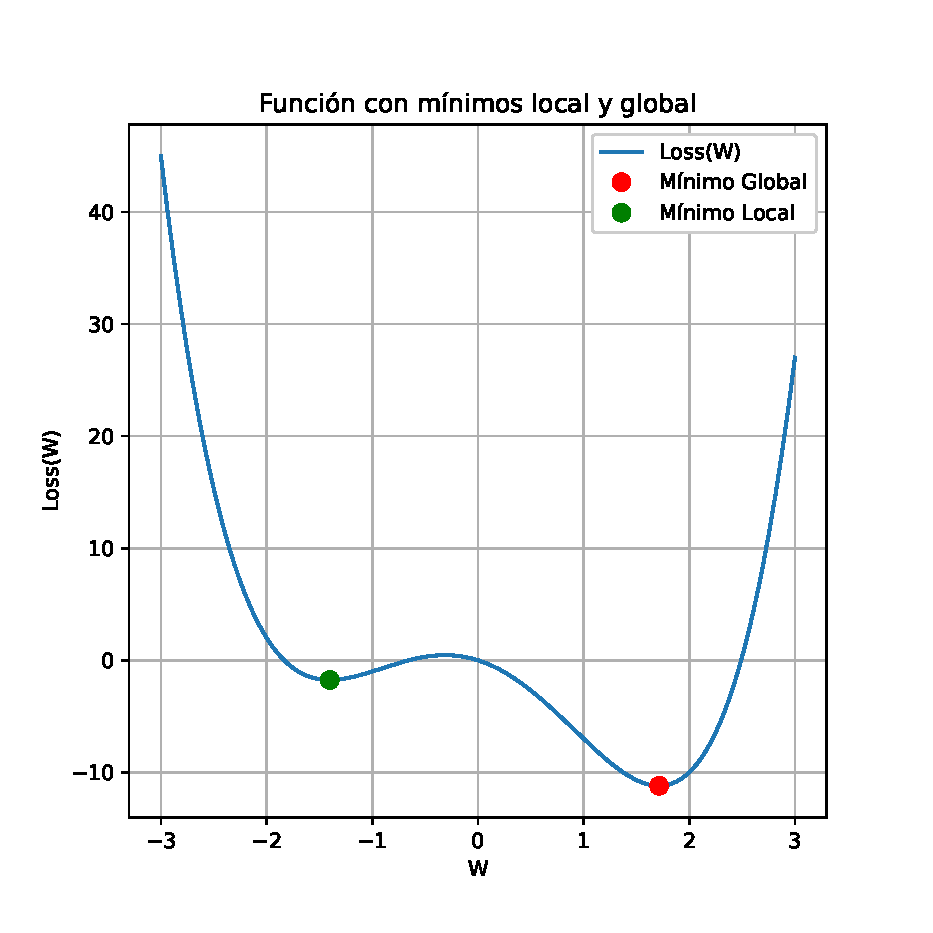
\includegraphics[height=0.65\textheight]{minimos}
	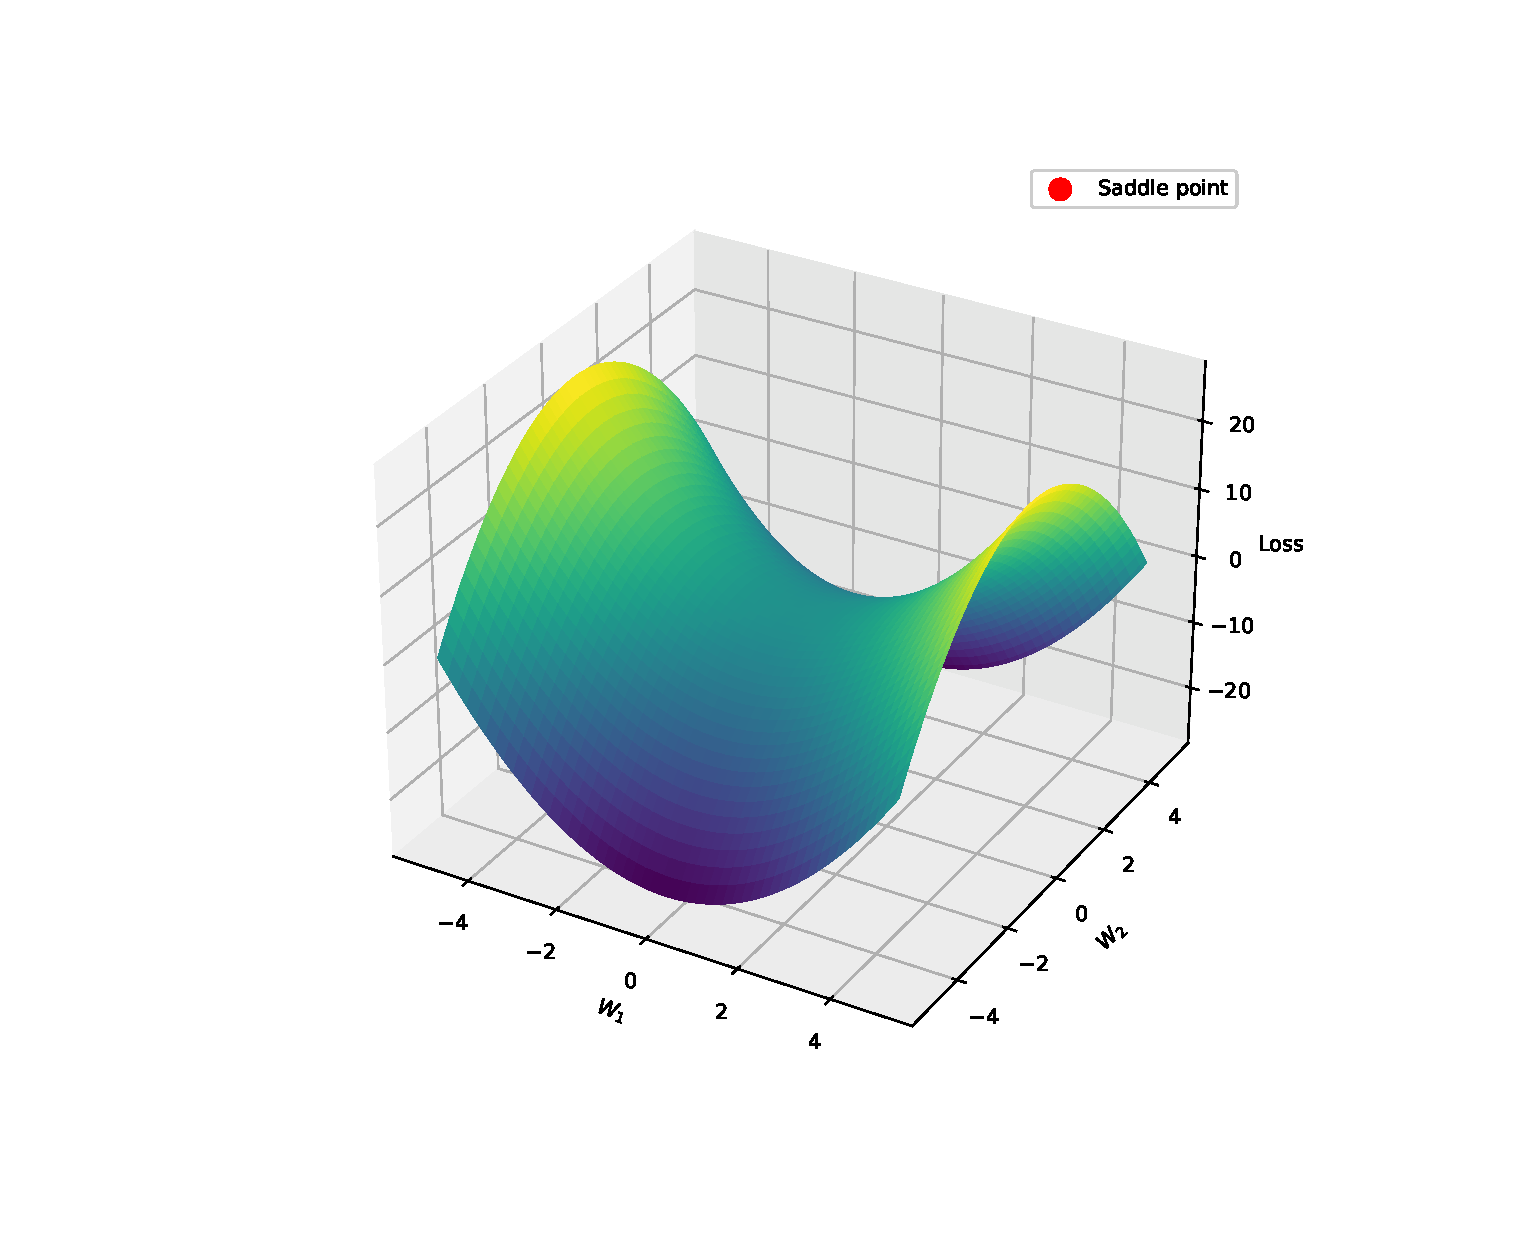
\includegraphics[trim={10 10 10 50}, clip, height=0.65\textheight]{saddle_point}
\end{center}
\end{itemize}
}


\frame{
	\frametitle{Goal of Optimization vs. Deep Learning}
	\begin{itemize}
		\item Optimization aims to \textbf{minimize the loss function} — usually computed on the training data.
		\item Deep learning aims to \textbf{find a model that generalizes well} to unseen data.
		\item Training error $\neq$ generalization error.
		\item Minimizing training loss alone may lead to \textbf{overfitting}.
		\item Successful learning balances optimization efficiency and generalization ability.
	\end{itemize}
}


\frame{
	\frametitle{Generalization and Risk Minimization}
	\begin{itemize}
		\item \textbf{Empirical Risk:} Average loss over the training dataset \footnote{$\theta(x)$ indicates the prediction of the network; $y$ the true label}.
		\begin{equation}
			\hat{R}(f) = \frac{1}{n} \sum_{i=1}^{n} \mathcal{L}(\Phi(x_i), y_i)
		\end{equation}
		
		
		\item \textbf{Expected Risk (True Risk):} Expected loss over the unknown data distribution.
		\begin{equation}
			R(f) = \mathbb{E}_{(x,y) \sim \mathcal{D}} [\mathcal{L}(\Phi(x), y)]
		\end{equation}
		
		
		\item Deep learning seeks to minimize expected risk, but we can only optimize empirical risk.
		\item \textbf{Generalization} refers to how close these two risks are.
	\end{itemize}
}


\frame{
\frametitle{Empirical risk optimization\footnote{Zhang, Aston, et al. Dive into deep learning. Cambridge University Press, 2023.}}
\begin{figure}
	\centering
	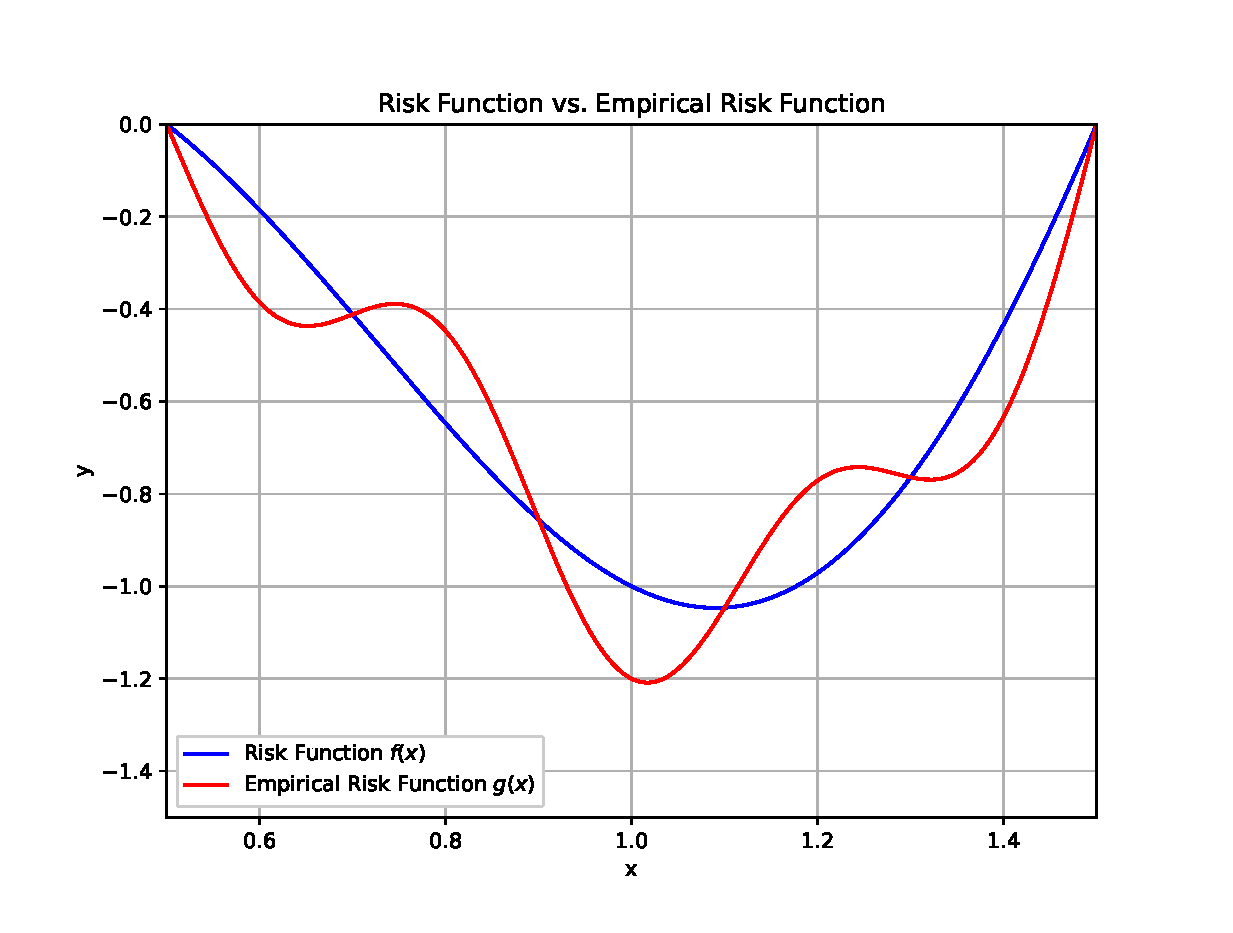
\includegraphics[height=0.6\textheight]{risk_vs_empirical_risk}
	\caption{Deep learning seeks to minimize risk, but we can only optimize empirical risk.}
	\label{fig:riskvsempiricalrisk}
\end{figure}
}


\section{Gradient Descent}

\begin{frame}
\frametitle{Gradient descent}
\begin{itemize}
\item Optimization algorithm that iteratively updates the parameters of a function.
\begin{equation}
	W_{\text{new}} = W_{\text{old}} - \eta \nabla_W \mathcal{L} (W, D)
\end{equation} where $\mathcal{L}$ is the loss function, $\eta$ the learning rate, $W$ the parameters of the model and $D$ the dataset.
\end{itemize}
\end{frame}


\begin{frame}
\frametitle{Example}
Spheric function.
\begin{equation}
f(x, y) = x^2 + y^2
\end{equation}

\begin{figure}
	\centering
	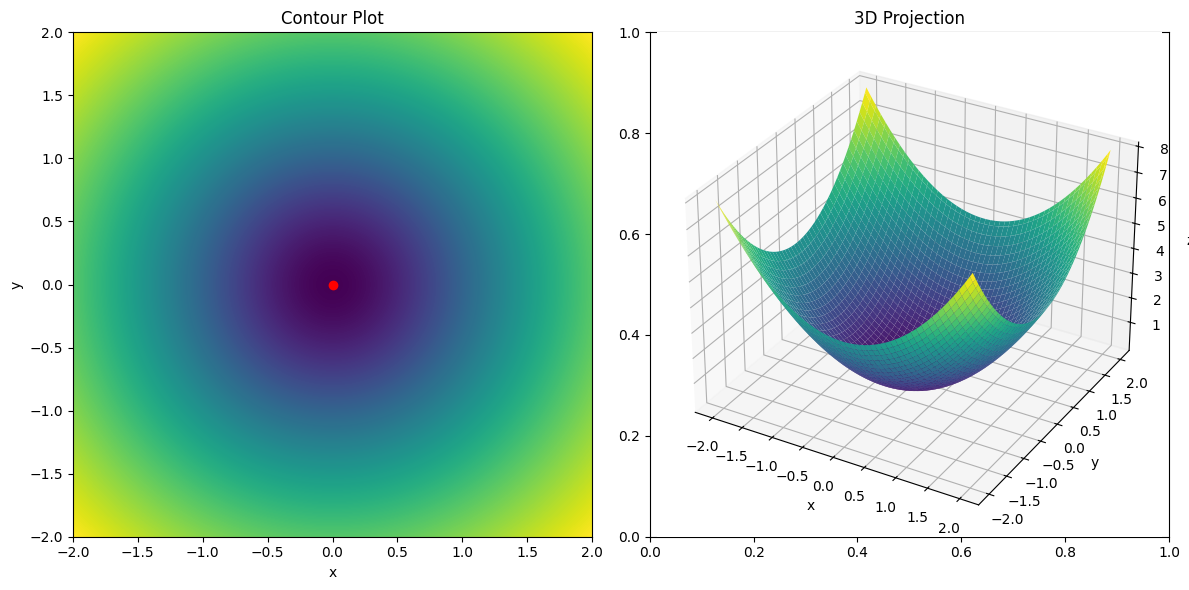
\includegraphics[height=0.6\textheight]{sphere}
%	\caption{}
%	\label{fig:sphere}
\end{figure}
\end{frame}


\begin{frame}
\frametitle{Example}
\begin{figure}
	\centering
	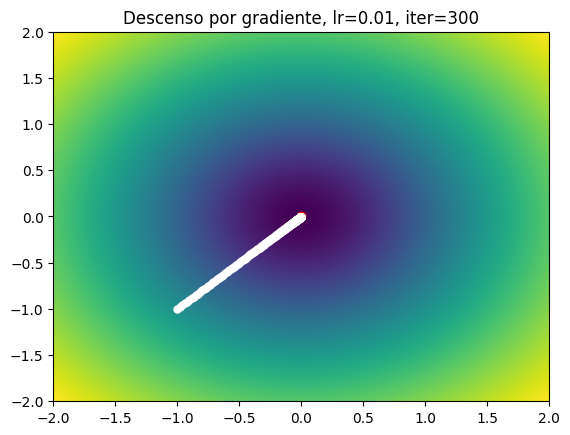
\includegraphics[height=0.7\textheight]{sol_dg}
	\caption{Solution to the sphere funcion.}
	\label{fig:soldg}
\end{figure}

\end{frame}




\begin{frame}
\begin{figure}
	\centering
	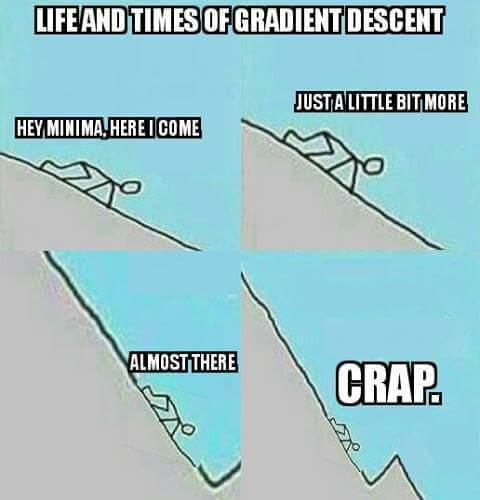
\includegraphics[height=0.8\textheight]{1577601074946}
	\caption{True story}
	\label{fig:1577601074946}
\end{figure}
\end{frame}



\section{Stochastic Gradient Descent}


\frame{
	\frametitle{Stochastic Gradient Descent (SGD)}
	\begin{itemize}
		\item For large datasets. We update the weights using a random set of tuples $(x_i,y_i)$, \textbf{Minibatch}. The algorithm achieves linear convergence \footnote{{\tiny Bottou L. (2012) Stochastic Gradient Descent Tricks. In: Montavon G., Orr G.B., Müller KR. (eds) Neural Networks: Tricks of the Trade. Lecture Notes in Computer Science, vol 7700. Springer, Berlin, Heidelberg.}.}
		\pause
		\begin{center}
			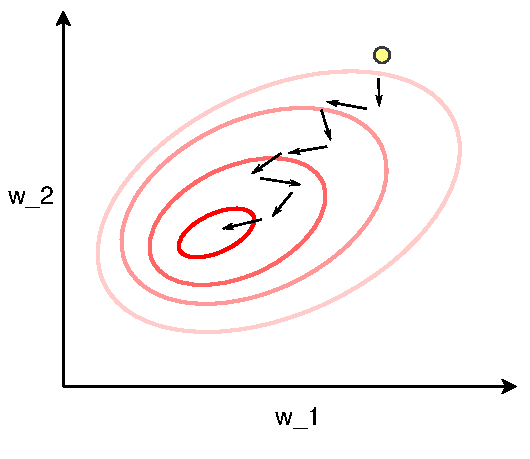
\includegraphics[height=0.55\textheight]{./sgd_a}
		\end{center}
	\end{itemize}
}


\frame{
	\frametitle{Batch Size}
	\begin{itemize}
		\item The batch size determines how many training examples are used in one iteration.
		\item Typical values: 32, 64, 128. Smaller batches add noise but can help escape local minima.
		\item Large batches converge faster but may get stuck in sharp minima.
	\end{itemize}
	
\begin{figure}
	\centering
	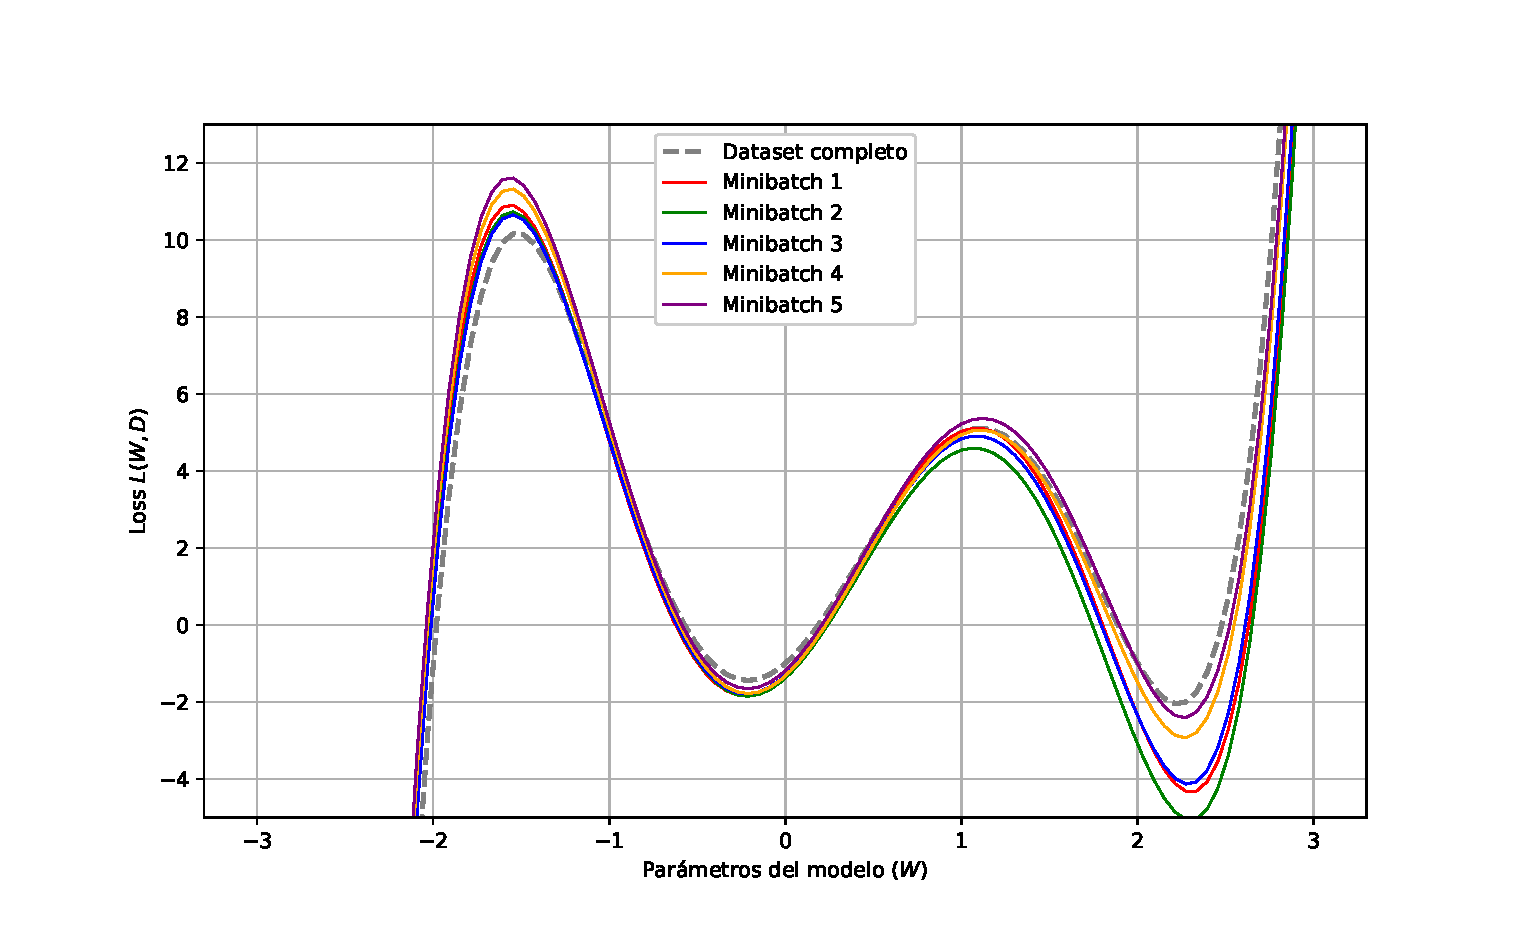
\includegraphics[height=0.6\textheight,trim={10 20 10 50}, clip]{full_vs_minibatches}
	\caption{Loss function for several datasets}
	\label{fig:fullvsminibatches}
\end{figure}
}



\frame{
	\frametitle{Batch Normalization}
	\begin{itemize}
		\item Normalizes inputs to each layer to have mean 0 and variance 1.
		\item Reduces internal covariate shift.
		\item Improves training stability and allows higher learning rates.
	\end{itemize}
}

\begin{frame}{So far so good}
\begin{figure}
	\centering
	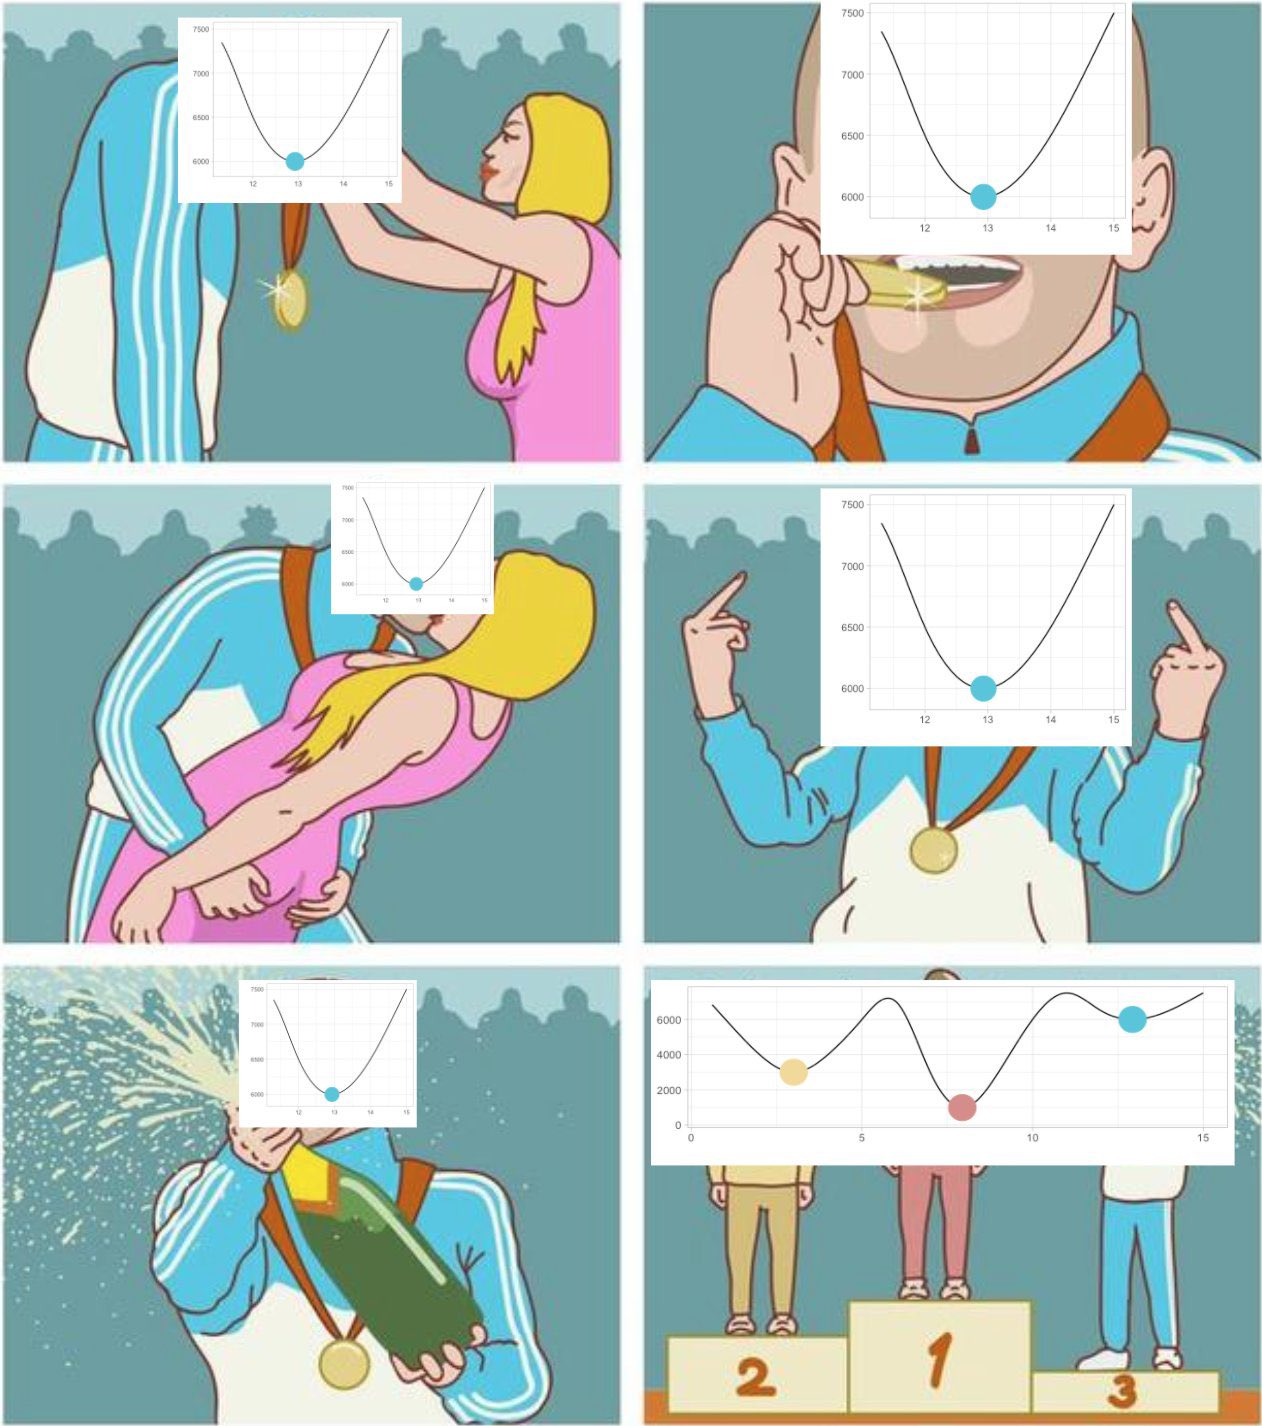
\includegraphics[height=0.75\textheight]{FSDfnEyUcAEUMSd}
	\caption{Stochastic gradient descent}
	\label{fig:fsdfneyucaeumsd}
\end{figure}
\end{frame}


%\frame{
%	\frametitle{Stochastic Gradient Descent (SGD)}
%	\begin{itemize}
%		\item Some tips
%		\item Inputs mean 0 and equal variance
%		\item Initial weights, random, mean 0 and small variance
%	\end{itemize}
%
%}


\section{Including Momentum}


\frame{
	\frametitle{SGD - Momentum}
	\begin{itemize}
		\item SGD may over sigzag
		\item The momentum can improve the efficiency.
		\begin{equation}
		M_t = \beta M_{t-1} + (1-\beta) \nabla_w \mathcal{L} (W, X, Y)
		\end{equation}
		\begin{equation}
		W_t = W_{t-1} - \eta M_t
		\end{equation}
		\pause
		\begin{center}
			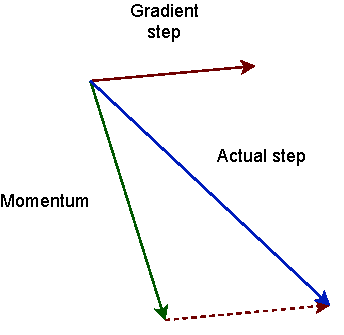
\includegraphics[height=0.45\textheight]{./momentum}
		\end{center}
		\item Usually $\beta$ = 0.9
	\end{itemize}
}


\frame{
	\frametitle{SGD - Momentum (2)}
	\begin{center}
		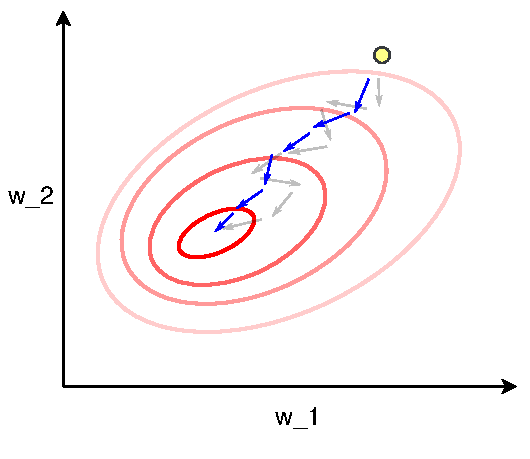
\includegraphics[height=0.65\textheight]{./sgd_M}
	\end{center}
}


\begin{frame}
	\frametitle{Example: Beale's function}
	\begin{itemize}
		\item La función de Beale es una función de prueba comúnmente utilizada en la optimización para evaluar el rendimiento de algoritmos en problemas no convexos.
		\begin{equation}
			f(x, y) = (1.5 - x + xy)^2 + (2.25 - x + xy^2)^2 + (2.625 - x + xy^3)^2
		\end{equation}
	\end{itemize}
\begin{figure}
	\centering
	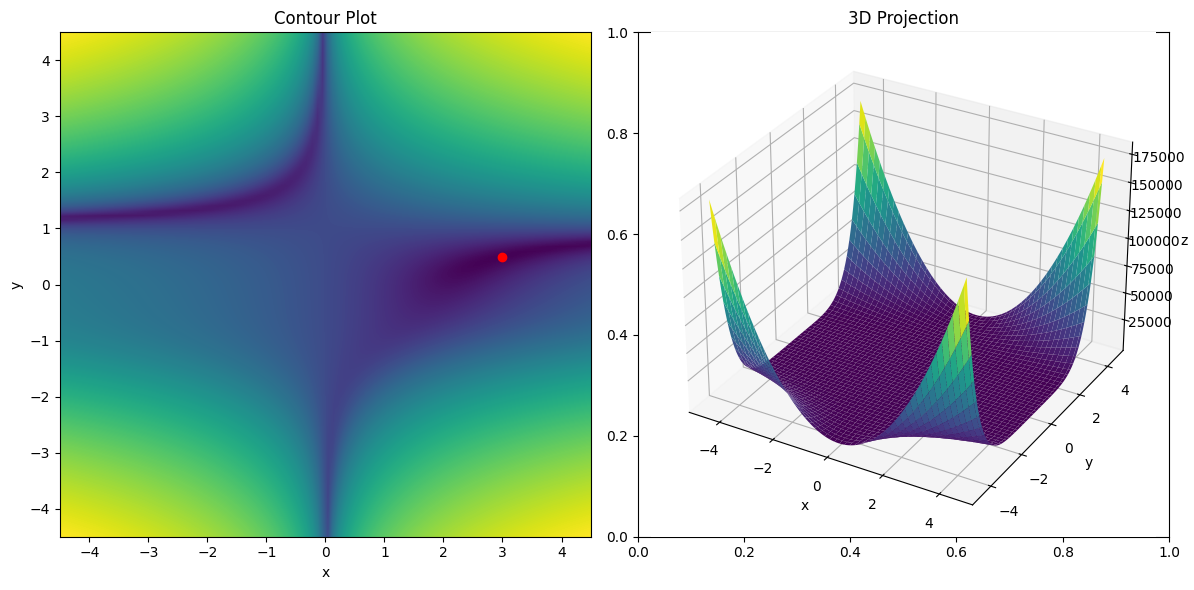
\includegraphics[height=0.5\textheight]{beale}
%	\caption{}
	\label{fig:beale}
\end{figure}
\end{frame}



\begin{frame}
	\frametitle{Example}
	% Subfigures 
	\begin{figure}
		\centering
		\begin{subfigure}{.5\textwidth}
			\centering
			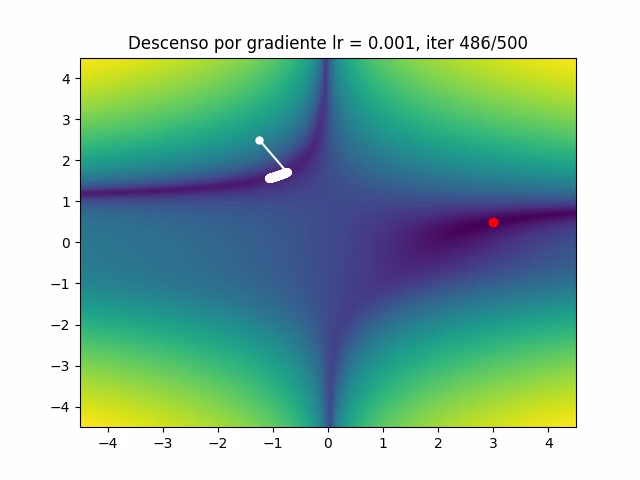
\includegraphics[height=0.7\textheight]{gradient_descent_beale}
			%\caption{A subfigure}
			%\label{fig:sub1}
		\end{subfigure}%
		\begin{subfigure}{.5\textwidth}
			\centering
			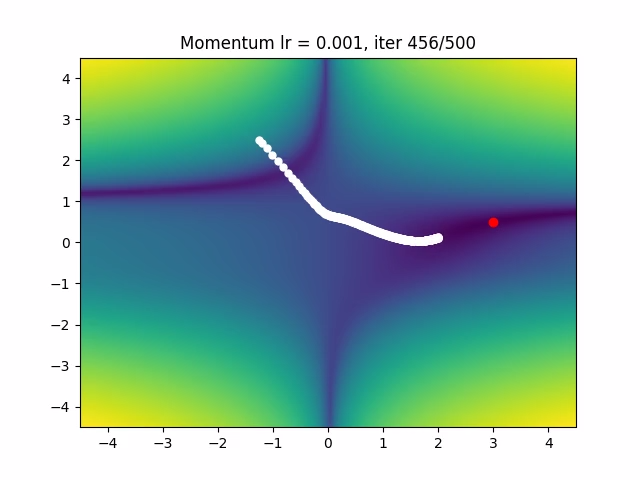
\includegraphics[height=0.7\textheight]{gradient_descent_momentum_beale}
			%\caption{A subfigure}
			%\label{fig:sub2}
		\end{subfigure}
		\caption{Performance of the optimization methods}
		\label{fig:test}
	\end{figure}
\end{frame}



%\frame{
%\frametitle{Learning Rate Decay}
%\begin{center}
%\includegraphics[width=\linewidth]{./lrdecay}
%\end{center}
%}






%\frame{
%	\frametitle{SGD - Momentum}
%	\pause
%	\begin{center}
%		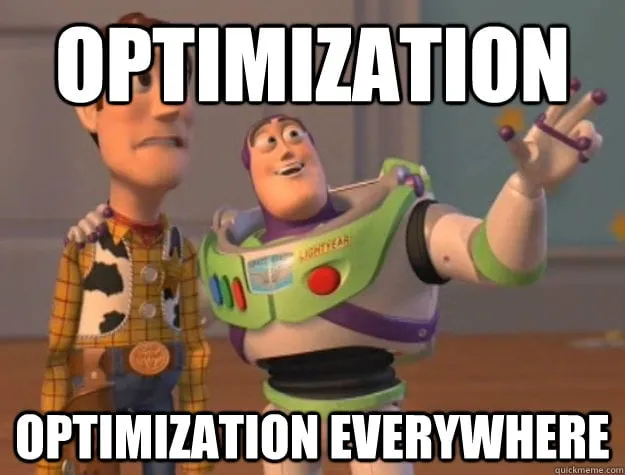
\includegraphics[height=0.7\textheight]{optimization-meme}
%	\end{center}
%}


\section{Adaptative gradient}


\begin{frame}
	\frametitle{Motivation}
\begin{figure}
	\centering
	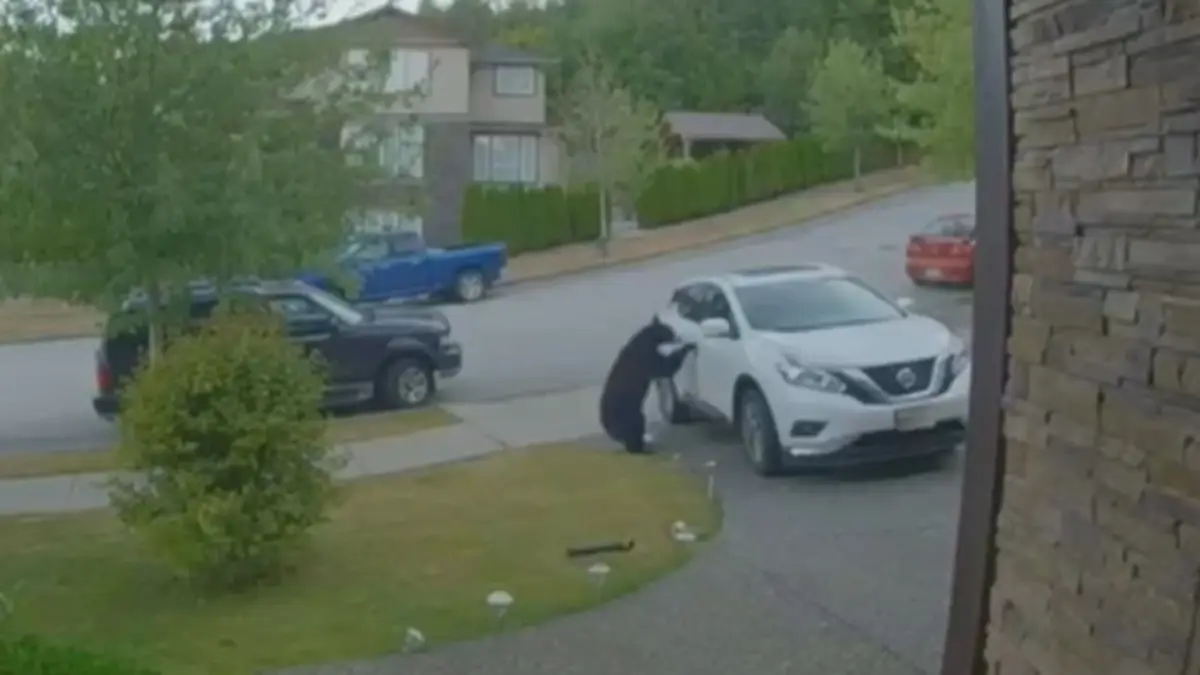
\includegraphics[height=0.7\textheight]{WEB_BEAR}
	\caption{Which are infrecuent features?}
	\label{fig:webbear}
\end{figure}
\end{frame}

	
\begin{frame}
		\frametitle{Optimizing for infrecuent features: Adagrad}
		
		\begin{itemize}
			\item The core problem: The learning rate decays too quickly for infrequent features (which need more updates) or too slowly for common features.
			
			\item Adagrad (Duchi et al., 2011) addresses this by providing an adaptive, per-parameter learning rate.
			
			\item Instead of using a crude update counter ($n_i$), Adagrad scales the learning rate for each parameter using the accumulated \textit{sum of the squares of its past gradients}.
			
			\item This mechanism automatically reduces the learning rate for parameters with large, frequent gradients and maintains a higher rate for parameters with small, infrequent gradients.
		\end{itemize}
\end{frame}



\frame{
\frametitle{AdaGrad \footnote{\scriptsize Duchi, John, Elad Hazan, and Yoram Singer. “Adaptive Subgradient Methods for Online Learning and Stochastic Optimization.” Journal of Machine Learning Research 12.Jul (2011): 2121-2159}}
\framesubtitle{Accumulation of gradients}
\begin{itemize}
	\item Adapts gradient over time using an accumulation of the historical gradients
	\item Initialization
	\begin{equation}
		r_0 = 0 	
	\end{equation}
	\item Accumulate the square of the gradients
	\begin{equation}
		r_i = r_{i-1} + g_i \odot g_i	
	\end{equation}
	\item Update
	\begin{equation}
		w_i = w_{i-1} - \frac{\eta}{k \oplus \sqrt{r_i}} \odot g_i
	\end{equation}
	where $k\approx 10^{
	-7}$ 
\end{itemize}
}


\frame{
\frametitle{RMSProp \footnote{\scriptsize Tieleman, T., \& Hinton, G. (2012). Rmsprop: Divide the gradient by a running average of its recent magnitude. Neural networks for machine learning. 17, 6.}}
\begin{itemize}
	\item RMSprop (Root Mean Square Propagation) improves over Adagrad.
	\item Adagrad + momentum
	\item Discards old measurements with $\rho$
	\begin{equation}
		r_i = \rho r_
		{i-1} + (1-\rho) g_i \odot g_i
	\end{equation}
	where $\rho$ determines how long we keep old gradients
	\item Update
	\begin{equation}
		w_i = w_{i-1} - \frac{\eta}{\sqrt{k \oplus r_i}} \odot g_i
	\end{equation}
	where $k\approx 10^{-7}$ 
\end{itemize}
}


\frame{
\frametitle{Adam \footnote{\scriptsize Adam, Kingma DP Ba J. "A method for stochastic optimization." arXiv preprint arXiv:1412.6980 1412.6 (2014).}}
\begin{itemize}
	\item Exponentially weighted moving average of the gradient (first momentum)
	\begin{equation}
		m_i = \beta_1 m_{i-1} + (1-\beta_1) g_i
	\end{equation}
	\item Moving average of the historical gradients (second momentum)
	\begin{equation}
		v_i = \beta_2 v_{i-1} + (1-\beta_2) g_i \odot g_i	
	\end{equation}
	\item Correction
	$$\tilde{m}_i =\frac{m_i}{1-\beta_1^i}$$
	$$\tilde{v}_i = \frac{v_i}{1-\beta_2^i}$$
	\item Update
	$$w_i = w_{i-1} - \frac{\eta}{k \oplus \sqrt{\tilde{v}_i}}\tilde{m}_i$$
\end{itemize}
}


\frame{
	\frametitle{Gradient Clipping}
	\begin{itemize}
		\item Prevents exploding gradients during backpropagation.
		\item Clip gradients to a threshold value:
		\begin{equation}
			\text{if } \|g\| > \tau, \quad g \leftarrow \tau \cdot \frac{g}{\|g\|}
		\end{equation}
		\item Especially useful in RNNs and deep networks.
	\end{itemize}
}


\frame{
\frametitle{What about the learning rate?}
\begin{center}
	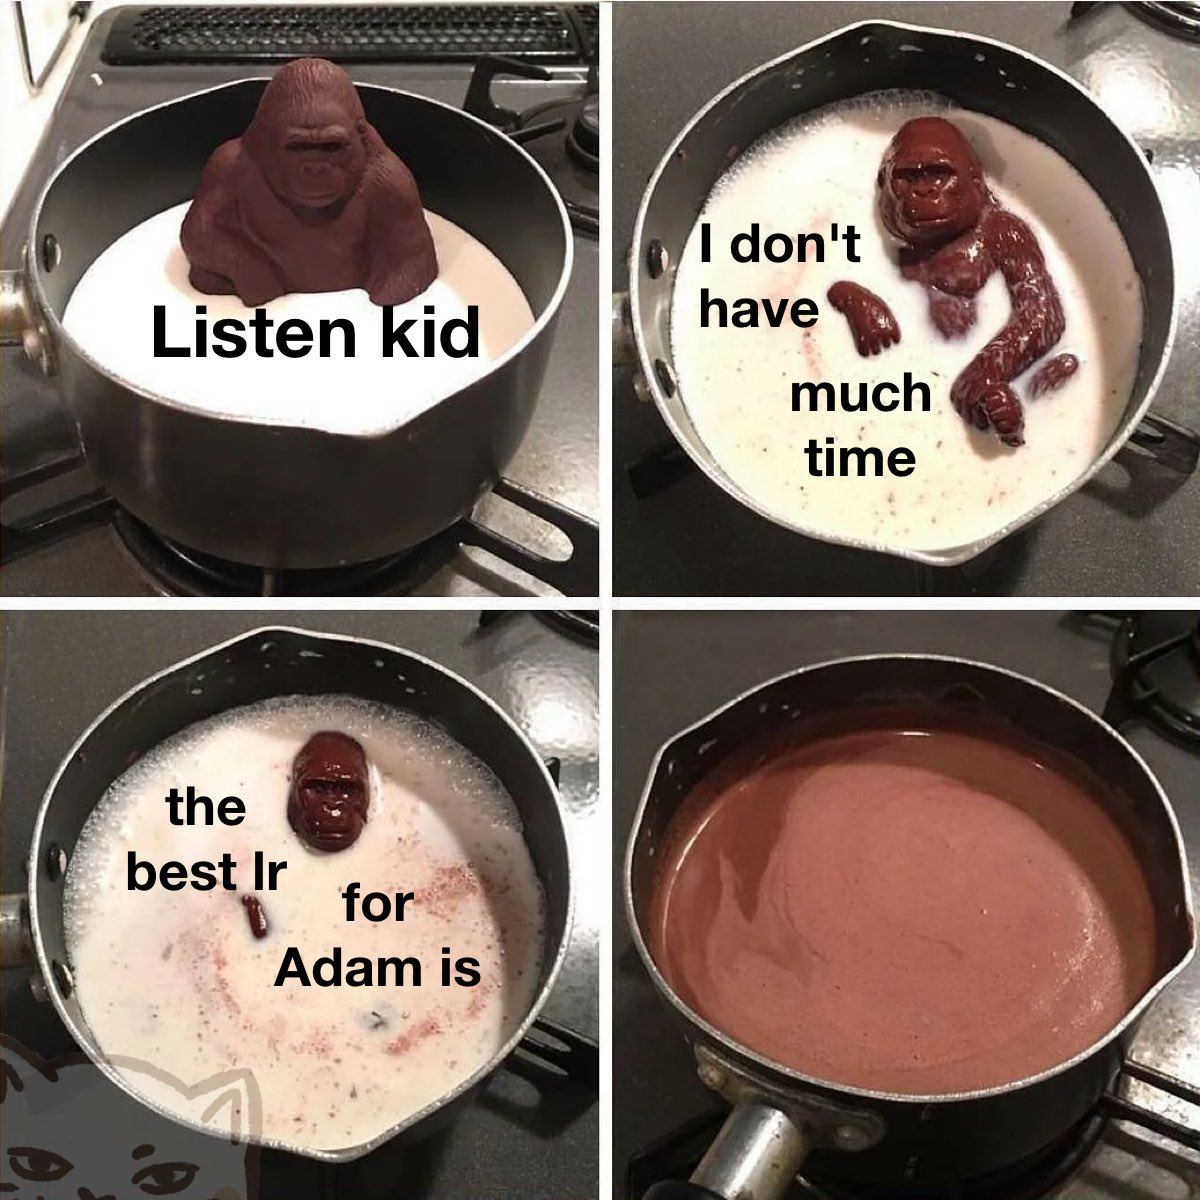
\includegraphics[height=0.8\textheight]{tip}
\end{center}
}


\section{Learning rate estimation}


\frame{
	\frametitle{Warm-up Strategy}
	\begin{itemize}
		\item Warm-up gradually increases the learning rate during the initial training phase \footnote{\scriptsize Kalra, Dayal Singh, and Maissam Barkeshli. "Why warmup the learning rate? underlying mechanisms and improvements." Advances in Neural Information Processing Systems 37 (2024): 111760-111801.}.
		\item Helps avoid instability due to large initial gradient updates.
		\item Often used with adaptive optimizers such as Adam.
		\item Linear warm-up:
		\begin{equation}
			\eta_t = \eta_{max} \cdot \frac{t}{T_{warmup}} \quad \text{if } t \leq T_{warmup}
		\end{equation}
	\end{itemize}
}


\frame{
	\frametitle{Learning Rate Decay}
	\begin{itemize}
		\item As we aproximate to the minimum the step may overshoot the target.
	\end{itemize}
	
	\begin{center}
		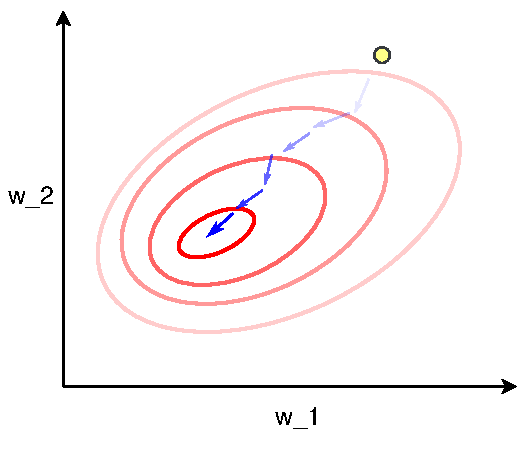
\includegraphics[height=0.65\textheight]{./lrd}
	\end{center}
}


\frame{
	\frametitle{Learning Rate Decay (2)}
	\begin{itemize}
		\item A solution is to apply a learning rate decay.
		\begin{equation}
			\eta = \eta_0 \left(  \frac{1}{1 + i d} \right) 
		\end{equation} where $\eta_0$ is the starting l.r., $i$ is the epoch and $d$ is the decay hyperparámeter.
	\end{itemize}
	
	\begin{figure}
		\centering
		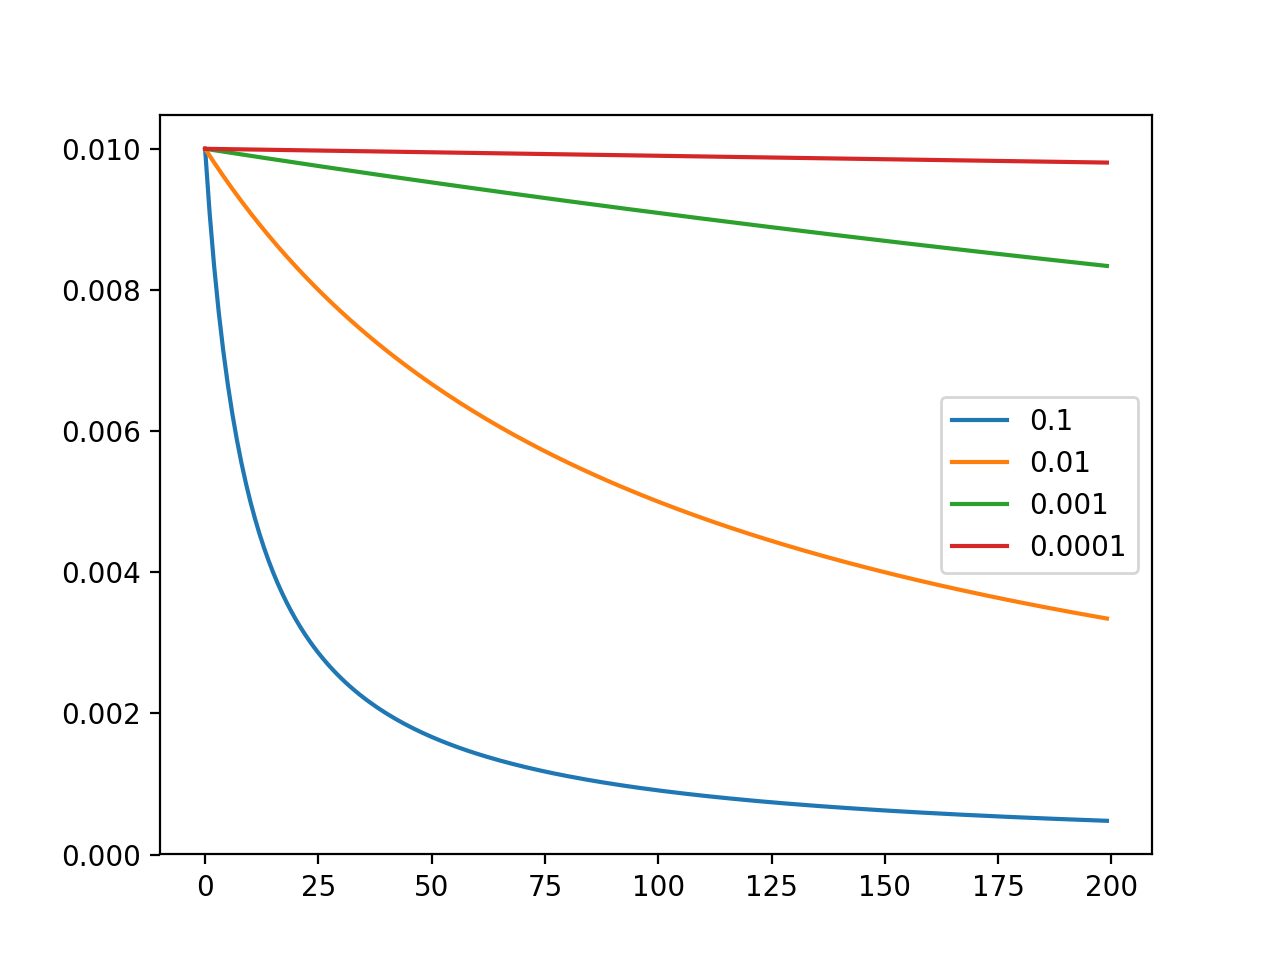
\includegraphics[height=0.5\textheight]{./d}
		\caption{Effect of the decay ($d$) on the learning rate.}
		\label{fig:d}
	\end{figure}
}


\frame{
	\frametitle{Optimizer selection}
	\begin{itemize}
		\item Consider them part of the design of experiment
		\item Currently, the main advances have been achieved by designing easy to train networks, instead of better optimizers
		\item Use Adam and improve the architecture
	\end{itemize}
}


\frame{
	\frametitle{Extra readings}
	\begin{itemize}
		\item \textbf{Chapter 4: Numerical Optimization.} Goodfellow, I., Bengio, Y., Courville, A., \& Bengio, Y. (2016). Deep learning (Vol. 1). Cambridge: MIT press.
		\item \textbf{Chapter 6: Beyond Gradient Descent.} Buduma, Nithin, Nikhil Buduma, and Joe Papa. Fundamentals of deep learning: Designing next-generation machine intelligence algorithms. " O'Reilly Media, Inc.", 2022.
	\end{itemize}
}


%\frame{
%\frametitle{References}
%\begin{itemize}
%   \item [Sucar 15] Sucar, Luis Enrique. Probabilistic Graphical Models: Principles and Applications. Springer, 2015.
%   \item [Smola] Alex Smola and S.V.N. Vishwanathan, Introduction to Machine Learning, Cambirdge University Press.
%   \item [Udacity] Self Driving Car Nanodegree
%   \item [Goodfellow] Goodfellow, I., Bengio, Y., Courville, A., \& Bengio, Y. (2016). Deep learning (Vol. 1). Cambridge: MIT press.
%\end{itemize}
%
%}


\end{document}